\documentclass[12pt,a4paper]{report}

\usepackage[T1]{fontenc}
\usepackage{titlesec, blindtext, color}
\definecolor{gray75}{gray}{0.75}
\newcommand{\hsp}{\hspace{20pt}}
\titleformat{\chapter}[hang]{\Huge\bfseries}{\thechapter\hsp\textcolor{gray75}{|}\hsp}{2pt}{\Huge\bfseries}
\usepackage{amsmath}



%adjust your page margins here
\usepackage[top=0.70in, bottom=0.70in, left=0.8in,right=0.80in]{geometry} % setting the page alignment with this package
\usepackage[pdftex]{graphicx} %for embedding images
\usepackage[%dvips, % commented for pdflatex
bookmarks,  colorlinks=false]{hyperref} %for creating links in the pdf version and other additional pdf attributes, no effect on the printed document
\hypersetup{%
    pdfborder = {0 0 0}
}
\usepackage[final]{pdfpages} %for embedding another pdf, remove if not required
\usepackage{float} %used for figure placement with H as a parameter
\usepackage{hyperref}
\usepackage{pslatex} % for times new roman, old package, but works
\usepackage{array} % for making text bold in table
\usepackage{setspace}
\usepackage{float}
\usepackage{enumerate}
\usepackage{longtable}

\usepackage[font=small,labelfont=bf]{caption}
\def\figurename{\textbf{Figure }}

\usepackage{listings}
\usepackage{color}

\definecolor{dkgreen}{rgb}{0,0.6,0}
\definecolor{gray}{rgb}{0.5,0.5,0.5}
\definecolor{mauve}{rgb}{0.58,0,0.82}
 
\lstset{ %
  language=Java,                % the language of the code
  basicstyle=\footnotesize,           % the size of the fonts that are used for the code
  numbers=left,                   % where to put the line-numbers
  numberstyle=\tiny\color{gray},  % the style that is used for the line-numbers
  stepnumber=1,                   % each line is numbered
  numbersep=5pt,                  % how far the line-numbers are from the code
  backgroundcolor=\color{white},      % choose the background color. You must add \usepackage{color}
  showspaces=false,               % show spaces adding particular underscores
  showstringspaces=false,         % underline spaces within strings
  showtabs=false,                 % show tabs within strings adding particular underscores
  frame=single,                   % adds a frame around the code
  rulecolor=\color{black},        % if not set, the frame-color may be changed on line-breaks within not-black text (e.g. commens (green here))
  tabsize=2,                      % sets default tabsize to 2 spaces
  captionpos=b,                   % sets the caption-position to bottom
  breaklines=true,                % sets automatic line breaking
  breakatwhitespace=false,        % sets if automatic breaks should only happen at whitespace
  title=\lstname,                   % show the filename of files included with \lstinputlisting;
                                  % also try caption instead of title
  keywordstyle=\color{blue},          % keyword style
  commentstyle=\color{dkgreen},       % comment style
  stringstyle=\color{mauve},         % string literal style
  escapeinside={\%*}{*)},            % if you want to add a comment within your code
  morekeywords={*,...}               % if you want to add more keywords to the set
}

%For the header and footer
\usepackage{fancyhdr}
\fancypagestyle{plain}{%
\fancyfoot[L]{\emph{Electrical Engineering , IIT-Bombay}} % except the center
\fancyfoot[R]{\thepage}
\renewcommand{\headrulewidth}{0.4pt}
\renewcommand{\footrulewidth}{0.4pt}
}

\pagestyle{fancy}

\rhead{\emph{Undergraduate Thesis}}

\fancyfoot[LO,L]{\emph{Electrical Engineering , IIT-Bombay}}
\cfoot{}
\fancyfoot[RO, R]{\thepage}
\renewcommand{\headrulewidth}{0.4pt}
\renewcommand{\footrulewidth}{0.4pt}
%For the header and footer Over

%Page Border
\usepackage{pgf}
\usepackage{pgfpages}

\pgfpagesdeclarelayout{boxed}
{
  \edef\pgfpageoptionborder{0pt}
}
{
  \pgfpagesphysicalpageoptions
  {%
    logical pages=1,%
  }
  \pgfpageslogicalpageoptions{1}
  {
    border code=\pgfsetlinewidth{2pt}\pgfstroke,%
    border shrink=\pgfpageoptionborder,%
    resized width=.95\pgfphysicalwidth,%
    resized height=.95\pgfphysicalheight,%
    center=\pgfpoint{.5\pgfphysicalwidth}{.5\pgfphysicalheight}%
  }%
}
\pgfpagesuselayout{boxed}
\setlength{\parindent}{1cm}
%GLOBAL SETTINGS OVER, DOCUMENT BEGINS
\begin{document}
\renewcommand\bibname{References}
\lhead{ }

%FROM HERE YOUR PAGES START GETTING ADDED

% includes the cover page

\pagenumbering{arabic}

\newpage
\begin{center}
\thispagestyle{empty}
\Large{\textbf{Undergraduate Project Report\\ \large{ON}}}\\[0.7cm]
\LARGE{\textsc {\textbf{`` Applications of Machine Learning to Communication Systems''}}}\\[0.5cm]
\vspace{0.5cm}

\begin{figure}[H]
  \centering
    
\includegraphics[height= 6.5cm, width=6.5
    cm]{project/images/IITBombay}
\end{figure}

\Large{\textbf{\\Submitted to}}
\LARGE{\textbf{\\Department of Electrical Engineering ,\\ Indian Institute of Technology -Bombay\\}}

\Large{\textbf{\\BY}}\\[0.5cm]
\Large{\textbf{Sujay Mundada}}\\[0.5cm]

\vspace{0.5cm}
\large{\textbf{UNDER THE GUIDANCE OF}}\\
\large{\textbf{Prof. Kumar Appaiah}}\\
\vspace{1cm}

\vspace{1cm}


\newpage
\end{center}
\newpage

% includes the acknowledgements page
\begin{center}
\thispagestyle{empty}
\LARGE{\textbf{Acknowledgements}}\\[1cm]
\end{center}
\linespread{1.13}
\large{} I'm profoundly thankful to professor Kumar Appaiah for helping and guiding me throughout this project
\newpage
 
\newpage

\begin{center}
\thispagestyle{empty}
\vspace{2cm}
\LARGE{\textbf{ABSTRACT}}\\[1.0cm]
\end{center}
\thispagestyle{empty}
\Large{}We present and discuss several novel applications of machine learning (ML) for the physical layer, by interpreting a communications system as an autoencoder and analyse the role of convolutional neural networks and deep neural networks on raw IQ samples for modulation classification.
\section*{Blind Pre-processor Modulation Classifier}
We tend to build a deep neural network to help classify modulation used to transmit the digital data before processing stage by using supervised learning and tend to show that they  outperform traditional classification techniques based on expert features. 
\vspace{-1cm}
\Large{}\paragraph{}
\section*{Modelling Communication Channels as Autoencoders}
\Large{}\paragraph{} We address the problem of learning an efficient and adaptive physical layer encoding to communicate binary information over an impaired channel. In contrast to traditional work, we treat the problem an unsupervised machine learning problem .We tend to reconstruct the wireless channel model as an end-to-end model that seeks to jointly optimize transmitter and receiver components in a single process.

\vspace{1cm}
\textbf{Keywords:} {Supervised Learning, Autoencoder, Unsupervised Learning, Modulation, Physical Layer } % adds the Research Methodology page
\newpage

%TABLE OF CONTENTS AND LIST OF FIGURES ARE AUTOMATICALLY ADDED BY FOLLOWING COMMANDS
%ADD FIGURE OF TABLES IF YOU NEED TO, CHECK DOCUMENTATION
 %numbering before main content starts


%To reset the Header & Footer for TOC and LOF
\pagestyle{empty}
\addtocontents{toc}{\protect\thispagestyle{empty}}
\tableofcontents % adds Index Page

\addtocontents{lof}{\protect\thispagestyle{empty}}
\listoffigures % adds List of Figures
\cleardoublepage

%And reset back the settings we choose for Header and Footer
\pagestyle{fancy}

\newpage
 %reset numbering to normal for the main content


\chapter{Introduction}
\paragraph{}Radio communication/wireless communication is all about finding efficient ways to transfer information over a channel which can be as simple as corruption with a Gaussian noise to more complex channels exhibiting features like multi-path fading, impulsive noise and so on. 
\paragraph{}Theoretically we often know the upper or lower bounds on various quantities like achievable capacity and information density vs bit error rates for given modulation schemes, bandwidths and signal to noise ratios etc. In practice we have been able to much closer to them but this usually involves a complex and expensive hardware support and DSP software tuning which may not be feasible in everyday practice.
\paragraph{}By taking approach of unsupervised and supervised learning we sought to optimize the reconstruction of a communication channel or classify modulation schemes at the preprocessor level. 

\section{Potential of ML for the physical layer}
\paragraph{} ML algorithms could provide improvement over existing physical layer algorithms. Most common models in wireless systems involve linear, stationary mathematical models and have Gaussian statistics. Real-life systems however have a lot of imperfections and non-linearities. For this reason deep learning bases systems can be optimized for a particular hardware configuration. Moreover most of the communication system models involve individual optimization of the various blocks involved in the transmission of the signal like source, channel, modulation, encoding, equalization. Although this system has given us very efficient models but it not entirely clear that making such individual components efficient will lead to best end-to-end performance. Attempts to jointly optimize these components as it done in machine learning however will guarantee us the best end-to-end performance. 


\section{Project Goal \& Specification}
\paragraph{}The goal of our project to look closely at 2 applications of machine learning in communication systems. The first one involves the classification of modulation at the pre-processor level, which will help us reduce the overhead in transmission of signals which usually involves encoding the type of modulation in the transmitted signal as well. The second application involves using unsupervised learning to model an end-to-end communications systems by optimization of both the trasnmitter and receiver model as one deep neural network that can be trained as an autoencoder to minimize the reconstruction loss and show that this achieves equivalent BLER compared to the traditional methods of hamming encoding.The beauty of this approach is that it can even be applied to channel models and loss functions for which the optimal solutions are unknown.

 % adds the introduction page
\chapter{Basics of Machine Learning}

\section{Types of machine learning}


\begin{equation}\nonumber
Machine Learning 
\begin{cases}
\text{Supervised learning} 
\begin{cases} 
\text{Classification} \\ 
\text{Regression} 
\end{cases}\\
\text{Unsupervised learning} 
\begin{cases}
\text{Discovering clusters} \\ 
\text{Discovering latent factors} \\ 
\text{Discovering graph structure} \\ 
\text{Matrix completion} 
\end{cases}\\
\end{cases}
\end{equation}


\section{Three elements of a machine learning model}
\paragraph{}Model = Representation + Evaluation + Optimization

\subsection{Representation}
\paragraph{}In supervised learning, a model must be represented as a conditional probability distribution $P(y|\vec{x})$ (usually we call it classifier) or a decision function $f(x)$. The set of classifiers(or decision functions) is called the hypothesis space of the model. Choosing a representation for a model is tantamount to choosing the hypothesis space that it can possibly learn. 


\subsection{Evaluation}
\paragraph{}In the hypothesis space, an evaluation function (also called objective function or risk function) is needed to distinguish good classifiers(or decision functions) from bad ones.


\subsection{Loss function and risk function}

\begin{definition}
In order to measure how well a function fits the training data, a \textbf{loss function} $L:Y \times Y \rightarrow R \geq 0$ is defined. For training example $(x_i,y_i)$, the loss of predicting the value $\widehat{y}$ is $L(y_i,\widehat{y})$.
\end{definition}

The following is some common loss functions:
\begin{enumerate}
\item 0-1 loss function \\ $L(Y,f(X))=\mathbb{I}(Y,f(X))=\begin{cases} 1, & Y=f(X) \\ 0, & Y \neq f(X) \end{cases}$
\item Quadratic loss function $L(Y,f(X))=\left(Y-f(X)\right)^2$
\item Absolute loss function $L(Y,f(X))=\abs{Y-f(X)}$
\item Logarithmic loss function \\ $L(Y,P(Y|X))=-\log{P(Y|X)}$
\end{enumerate}

\begin{definition}
The risk of function $f$ is defined as the expected loss of $f$:
\begin{equation}\label{eqn:expected-loss}
R_{\mathrm{exp}}(f)=E\left[L\left(Y,f(X)\right)\right]=\int L\left(y,f(x)\right)P(x,y)\mathrm{d}x\mathrm{d}y
\end{equation}
which is also called expected loss or \textbf{risk function}.
\end{definition}

\begin{definition}
The risk function $R_{\mathrm{exp}}(f)$ can be estimated from the training data as
\begin{equation}
R_{\mathrm{emp}}(f)=\dfrac{1}{N}\sum\limits_{i=1}^{N} L\left(y_i,f(x_i)\right)
\end{equation}
which is also called empirical loss or \textbf{empirical risk}.
\end{definition}

You can define your own loss function, but if you're a novice, you're probably better off using one from the literature. There are conditions that loss functions should meet:
\begin{enumerate}
\item They should approximate the actual loss you're trying to minimize. As was said in the other answer, the standard loss functions for classification is zero-one-loss (misclassification rate) and the ones used for training classifiers are approximations of that loss.
\item The loss function should work with your intended optimization algorithm. That's why zero-one-loss is not used directly: it doesn't work with gradient-based optimization methods since it doesn't have a well-defined gradient (or even a subgradient, like the hinge loss for SVMs has).

The main algorithm that optimizes the zero-one-loss directly is the old perceptron algorithm.
\end{enumerate}

\subsection{Optimization}
Finally, we need a \textbf{training algorithm}(also called \textbf{learning algorithm} ) to search among the classifiers in the the hypothesis space for the highest-scoring one. The choice of optimization technique is key to the \textbf{efficiency} of the model.

\section{Machine Learning Libraries}
\paragraph{}In recent times, numerous tools and algorithms have emerged that make it easy to build and train large NNs. Tools to deploy such training routines from high level language to massively parallel GPU architectures have been key enablers. Among these are Caffe, MXNet, TensorFlow, Theano, and Torch (just to name a few), which allow for high level algorithm definition in various programming languages. We have used tensorflow to code the NNs in this paper. 



 %adds details about ECG Signal
\chapter{Communication Channel as Autoencoder}

\section{Introduction}
In its simplest form, a communications system consists of a transmitter, a channel, and a receiver, as shown in Fig. 3.1.
\begin{figure}[H]
  \centering
    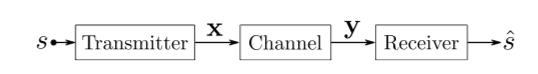
\includegraphics[height= 2cm, width=18cm]{project/images/channel.png}
  \caption{\textbf{Simple Communication Channel Model}}
\end{figure}
The transmitter wants to communicate one out of M possible messages s : M = {1,2,...,M} to the receiver making n discrete uses of the channel. To this end, it applies the transformation f to the message s to generate the transmitted signal x = f(s).The communication rate of this communications system is R = k/n, where k = log2(M). In the sequel, the notation (n,k) means that a communications system sends one out of M = 2k messages (k bits) through n channel uses.\\
From a DL point of view, this simple communications system can be seen as a particular type of autoencoder. Typically, the goal of an autoencoder is to find a low-dimensional representation of its input at some intermediate layer which allows reconstruction at the output with minimal error. In this way, the autoencoder learns to non-linearly compress and reconstruct the input. In our case, the purpose of the autoencoder is different. It seeks to learn representations x of the messages s that are robust with respect to the channel impairments mapping x to y (i.e., noise, fading, distortion, etc.), so that the transmitted message can be recovered with small probability of error. In other words, while most autoencoders remove redundancy from input data for compression, this autoencoder often adds redundancy, learning an intermediate representation robust to channel perturbations. The simple scheme of our autoencoder is shown in fig. 3.2
\vspace{3cm}
\begin{figure}[H]
  \centering
    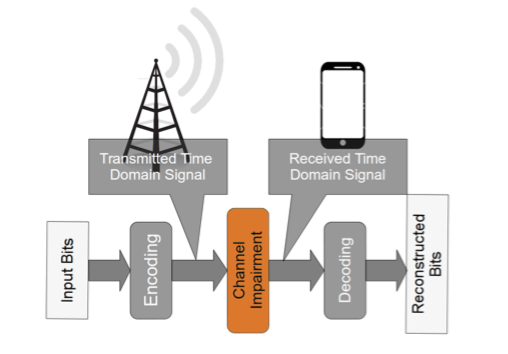
\includegraphics[height= 12cm, width=18cm]{project/images/encoder-decoder.png}
  \caption{\textbf{Modelling the channel as an Autoencoderl}}
\end{figure}

\newpage
\section{Implementation}
We constructed a new gaussian noise layer that adds a random normal noise to the transmitted signal. \\
The network works as is shown if fig. 3.3 and the parameters of the network built are shown in fig. 3.4 where M = 16 and n =128. 

\begin{figure}[H]
  \centering
    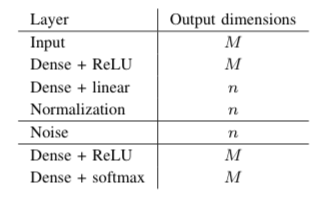
\includegraphics[height= 6cm, width=10cm]{project/images/network.png}
  \caption{\textbf{Autoencoder Network}}
\end{figure}

\begin{figure}[H]
  \centering
    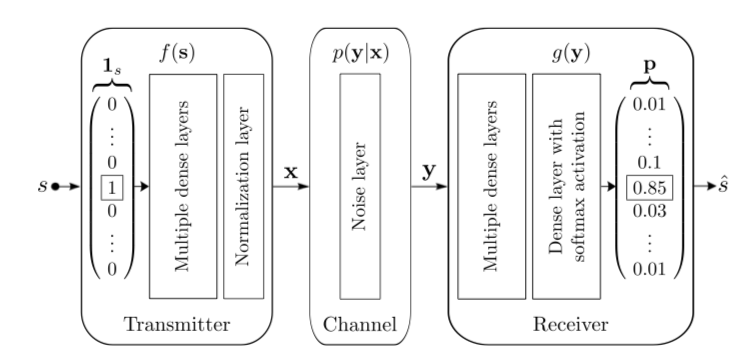
\includegraphics[height= 8cm, width=18cm]{project/images/statisticsOfNetwork.png}
  \caption{\textbf{Network Parameters}}
\end{figure}

\newpage
\section{Problems Faced}
The training was done and tested at a particular SNR but the results were not matching as proposed in the paper. We expected the performance of our autoencoder to match with that of hamming encoder with MLD decoding as shown in the below graph. 

\begin{figure}[H]
  \centering
    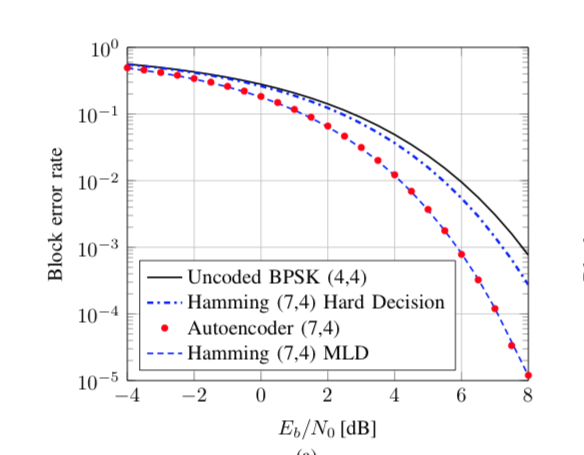
\includegraphics[height= 12cm, width=14cm]{project/images/graph.png}
  \caption{\textbf{Modelling the channel as an Autoencoderl}}
\end{figure} % adds Individual Subsystems
\chapter{Blind Pre-Processor Classifier}

\section{Introduction}
Modulation classification can be defined as the process of determining the modulation scheme of a noisy signal from a given set of possible schemes. This process has many applications in wireless communications, including in autonomous multimode and software defined radios. In most scenarios of interest, the difficulty in performing modulation classification is due primarily to the fact that classifiers operate with no or incomplete knowledge of the fading experienced by the signal and the distribution of the noise added in the channel. This is because a receiver typically has to first classify the received signal before it can successfully acquire symbol timing and estimate the channel state.The modulation classification operation can typically be divided into two stages. In the first, referred to as the pre- processing stage, the signal is acquired and different channel state and noise distribution parameters are estimated. With the obtained estimates, the signal is then classified in the second stage using an appropriate classification algorithm.

\newpage
\section{Applications}
Modulation classification was first motivated by its application in military scenarios where electronic warfare, surveillance and threat analysis requires the recognition of signal modulations in order to identify adversary transmitting units, to prepare jamming signals, and to recover the intercepted signal.\\
Link adaptation (LA), also known as adaptive modulation and coding (AM\&C), creates an adaptive modulation scheme where a pool of multiple modulations are employed by the same system. It enables the optimization of the transmission reliability and data rate through the adaptive selection of modulation schemes according to channel conditions. While the transmitter has the freedom to choose how the signals are modulated, the receiver must have the knowledge of the modulation type to demodulation the signal so that the transmission can be successful.\\
An easy way to achieve that is to include the modulation information in each signal frame so that the receivers would be notified about the change in modulation scheme,and react accordingly. However, this strategy affects the spectrum efficiency and throughput due to the extra modulation information in each signal frame. In the current situation where the wireless spectrum is extremely limited and valuable, the aforementioned strategy is simply not efficient enough. For this reason, pre-processor classification becomes an attractive solution to the problem.

\newpage
\section{Implementation}
We have used deep neural network(DNN) for the classification task. In DNN neurons are organized into layers: input, hidden and output. The input layer is composed not of full neurons, but rather consists simply of the record's values that are inputs to the next layer of neurons which are the I and Q components of the modulated received signal in our case. The next layer is the hidden layer. Several hidden layers can exist in one neural network, our network consists of 3 hidden layers with 256 neurons each. The final layer is the output layer, where there is one node for each class, 2 for our case. A single sweep forward through the network results in the assignment of a value to each output node which can be thought of as probability of detecting each class, and thus the record is assigned to the class node with the highest value probability. 

\subsection{Data Set Generation \& Representation}
The data set was generated using Octave. The data set comprises of 20000 data points each having 3 fields (I component, Q component and modulation class)

\subsection{Training \& Loss Functions}
The original data set is divided into 80 percent for training and 20 percent for testing. \\
The batch size is 500 with 2000 iterations each and learning rate used is 0.001 .\\
Loss function used is cross entropy loss function. 

\newpage
\section{Results \& Observation}
We obtained 100 percent classification for classification of QPSK vs 16QAM. \\ 
Using the channel model y= Hx + n given H we could use the same model with new training to obtain the same percentage classification. If H changes slowly with time as it happens practically we could train the old model using as fewer as 100 iterations and still obtain the same results.



\section{Future Work}

\begin{itemize}
    \item Extend the model to together classify all the most frequently used 9 digital and 2 analog modulation techniques.
    \item Try to train the network for a worse case impulsive noise training data and test for the gaussian noise cases.
    \item Tap the individual hidden layers to find out what features are they extracting at each level. 
    \item Use multiple samples of the same transmitted symbol and use Convolutional neural network to classify thereby using the correlation property between different samples of the same bit transmitted.
    \item Try to use progressive learning so that the the system to predict the change of channel matrix H 
\end{itemize} %general implementation
\chapter{Open Research Challenges}

In order to compare the performance of ML models and algorithms, it is crucial to have common benchmarks and open datasets. While this is the rule in the computer vision,voice recognition, and natural language processing domains (e.g., MNIST10 or ImageNet11), nothing comparable exists for communications. This domain is somewhat different because it deals with inherently man made signals that can be accurately generated synthetically, allowing the possibility of standardizing data generation routines rather than just data in some cases. It would be also desirable to establish a set of common problems and the corresponding datasets (or data-generating software) on which researchers can benchmark and compare their algorithms. One such example task is modulation classification ; others could include mapping of impaired received IQ samples or symbols to codewords or bits. % adds Individual Subsystems


\end{document}